\documentclass[./\jobname.tex]{subfiles}
\begin{document}
\section{Limitations}
This work and its proposed solver suffer from several limiting factors. At first, the testbed only includes one type of equation. Further, the treatment of the boundary condition is critically examined. Finally, the achieved quality is strictly limited by the \gls{nfe}-budget. Thus, the different algorithms are compared with their computational effort. 

\subsection{Testbed}

Contrary to the testbed used by other authors, the test-equations used here are only second order \gls{pde}s in $\mathbb{R}^2$. In particular, for all test-\gls{pde}s the Laplace operator $\Delta$ is applied to a solution function $u(\mathbf{x})$, resulting in various types of Poisson equations. Further, only Dirichlet type boundary conditions are used. This means that the testbed is not very diverse. Especially compared to \cite{chaquet_using_2019}, the testbed falls short of \gls{ode} and systems of differential equations. However, the results presented in the experiment chapters already indicate mixed performances on different testbed \gls{pde}s. Thus, starting with a manageable variety of problems helps with assessing the performance on a particular subset of differential equations.  


\subsection{Fulfilment of Boundary Condition}
Contrary to the \gls{fem} solver, the described \gls{ci} solver does not guarantee the boundary-condition fulfilment. There are ways to counteract the deviance on the boundary. 

A simple possibility is to increase the penalty factor $\varphi$ on the boundary collocation points $n_B$. This sets an emphasis on the boundary, however it still does not assure the fulfilment of the boundary condition.

As described in the literature overview, \cite{kirstukas_hybrid_2005} propose a strategy that repairs the boundary condition after the solver supposed an approximation to the interior domain. Introducing this strategy benefit the performance of the present solver. 

As discussed in chapter \ref{chap:testbed_description}, \gls{pde} 0A is used in the testbed by \cite{chaquet_using_2019} and \cite{mitchell_nist_2018}. Since preliminary experiments have shown that the \gls{ci} solver produced worse results on the \cite{mitchell_nist_2018} implementation, this version is adopted for the current testbed. The main difference between these variants of \gls{pde} 4 is the definition of the boundary condition: 

\begin{itemize}
	\item \underline{\textbf{\cite{mitchell_nist_2018}}}: 
	\begin{equation*}
		\begin{split}
		\text{Homogeneous Dirichlet Boundary Condition:} \\
		u(x,0) = 0 \\
		u(x,1) = 0 \\
		u(0,y) = 0 \\
		u(1,y) = 0 \\
		\end{split}
	\end{equation*}
	\item \underline{\textbf{\cite{chaquet_using_2019}}}:
	\begin{equation*}
		\begin{split}
		\text{Mixed Boundary Condition:} \\
		u(x,0) = 0 \\
		\frac{\partial u}{\partial y} (x,0) = \pi sin(\pi x) \\
		u(0,y) = 0 \\
		u(1,y) = 0 \\
		\end{split}
	\end{equation*}
\end{itemize}

Experiment 1 investigates the error behaviour of \gls{pde} 0A. As seen in figure \ref{fig:serial_parallel_pde4_error_comparison}, the error is large on the boundary of the domain $\partial \Omega$, while the interior suffers of a relatively small error. Thus, improvements on the boundary can be achieved more easily. Therefore, it makes sense that the solver is sensitive to the implementation of the boundary condition. However, in the typical application the boundary condition can not be rewritten. Thus, better methods for ensuring the boundary condition are needed. 


\subsection{Computational Effort}
\label{chap:computational_effort}

The greatest limiting factor for the solver is the extensive computational effort. This is best measured by the \gls{erd}. The \gls{erd} calculates the performance of heuristic optimisation algorithms and makes them comparable. \gls{erd} plots are often used in \gls{bbob} contests, such as the annual \gls{coco} workshop (\cite{nikolaus_hansen_2019_2594848}). A similar plot is shown in figure \ref{fig:ert_plot} below. 

The \gls{erd} plot shows the correlation between the \gls{nfe} and the percentage of the solved functions in the testbed. Therefore, the \gls{nfe} is increased from $10^3$ to $10^6$. The testbed consists of 11 \gls{pde}s. Further, different target values in the L2 norm are inspected: $5\cdot 10^{-2}$, $1\cdot 10^{-2}$, $5\cdot 10^{-3}$ and $1\cdot 10^{-3}$. Thus, the vertical axis indicates how often a algorithm reaches these $4 \cdot 11 = 44$ target values. 

\begin{figure}[H]
	\centering
	\noindent\adjustbox{max width=0.8\linewidth}{
		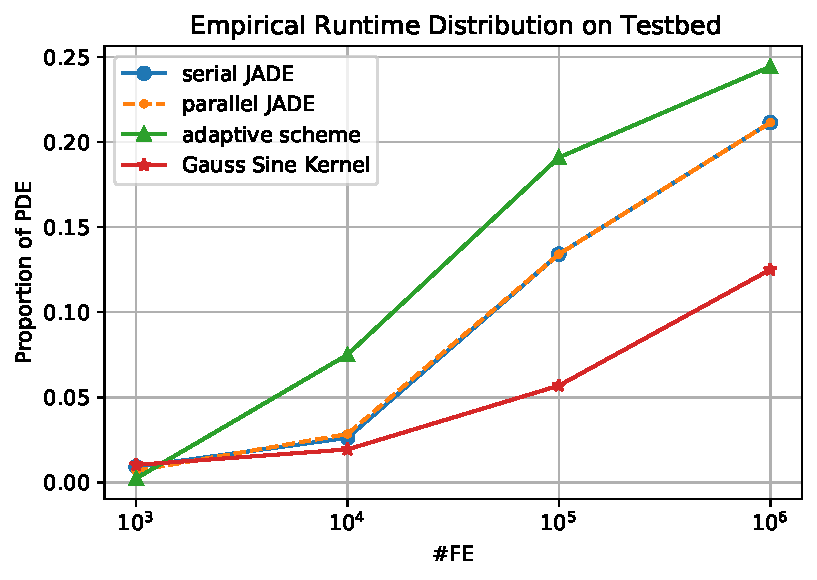
\includegraphics[width=\textwidth]{../../code/experiments/misc/ert_plot.pdf}
	}
	\unterschrift{Empirical Runtime Distribution of all algorithms on the 11 testbed \gls{pde}s at target values $5\cdot 10^{-2}$, $1\cdot 10^{-2}$, $5\cdot 10^{-3}$ and $1\cdot 10^{-3}$.}{}{}
	\label{fig:ert_plot}
\end{figure}

Remarkable is the virtually non-existing performance difference between the serial and the parallel memetic JADE. Since ``performance'' in this graph does not mean ``time-consumption'', this is expected.

The adaptive JADE scores continuously best and solves up to a quarter of the target values. This is largely thanks to the good performance on \gls{pde} 0A, which contributes 9 percent ($\frac{1}{11}$) to the whole testbed.  

Extrapolating the \gls{erd} plots indicates a further performance increase with more \gls{nfe}. Due to the already expensive algorithm, this is not tested. Substituting JADE for a faster converging algorithm might provide more clues to that matter. 


\end{document}